\chapter{Исследовательская часть}
В этом разделе будет продемонстрирована работа программы, а также
приведены результаты тестирования алгоритмов.

\section{Демонстрация работы программы}
На рисунке 4.1 приведена демонстрация работы программы.

\FloatBarrier
\begin{figure}[h]
	\begin{center}
		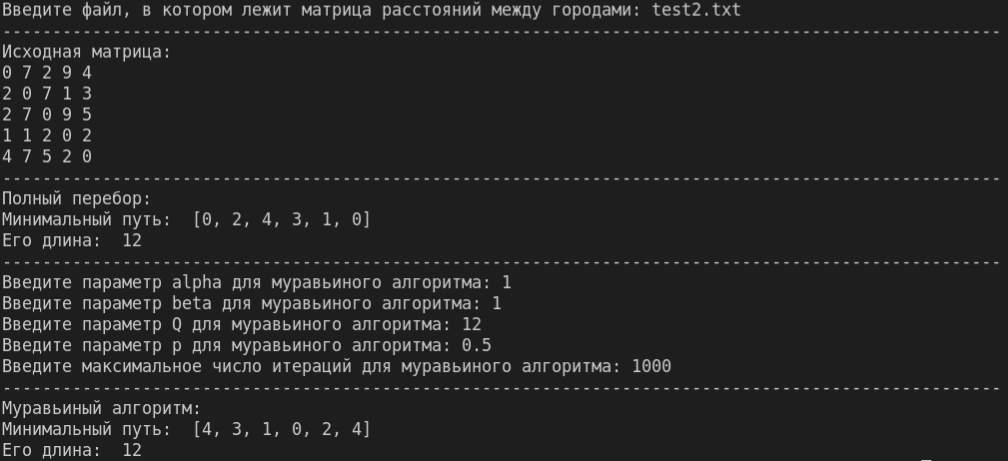
\includegraphics[]{inc/demonstrate.png}
	\end{center}
	\caption{Демонстрация программы}
\end{figure}
\FloatBarrier


\section{Технические характеристики}
Технические характеристики устройства, на котором выполнялось тестирование, следующие:
\begin{itemize}
	\item операционная система: Ubuntu 20.04.1 LTS;
	\item память: 8 GB;
	\item процессор: Intel Core i5-1135G7 @ 2.40GHz \cite{intel}.
	\item количество ядер процессора: 8
\end{itemize}

Во время тестирования ноутбук был нагружен только встроенными приложениями окружения, а также непосредственно системой тестирования.

\section{Тестирование программы}
Тестирование будет производиться в два этапа.

На первом этапе будет измерено время работы алгоритмов в зависимости от размера матрицы.
Параметры для муравьиного алгоритма стандартные: коэффициенты alpha и beta равны 1, Q = 10, а p = 0.5. 
Число итераций муравьиного алгоритма -- 1000.

На втором этапе будет протестирована работа муравьиного алгоритма в зависимости от параметров.
Будет проанализирован конечный ответ и итоговая ошибка алгоритма.
Будет использована матрица 15х15.

В таблице 4.1 представлены результаты первого этапа тестирования. 
Все алгоритмы выдавали один и тот же результат при всех размерах матрицы. 
\FloatBarrier
\begin{table}[h]
	\caption{Результаты тестов}
	\centering
	\begin{tabular}{ | l | l | l |}
		\hline
		Размер матрицы & Перебор & Муравьиный алгоритм\\ 
		\hline
		2 & 97774 & 26896807 \\
		3 & 56545 & 52780514 \\
		4 & 96257 & 84012718 \\
		5 & 174203 & 140044655 \\
		6 & 1493556 & 181273911 \\
		7 & 10373570 & 254475702 \\
		8 & 71372341 & 344602604 \\ 
		9 & 565912635 & 435430808 \\
		10 & 6325175130 & 619145862 \\ 
		11 & 75224132010 & 911105412 \\
		\hline
	\end{tabular}
\end{table}
\FloatBarrier

На рисунке 4.2 показан график зависимости времени работы алгоритмов от размера матрицы.

\FloatBarrier
\begin{figure}[h]
	\begin{center}
		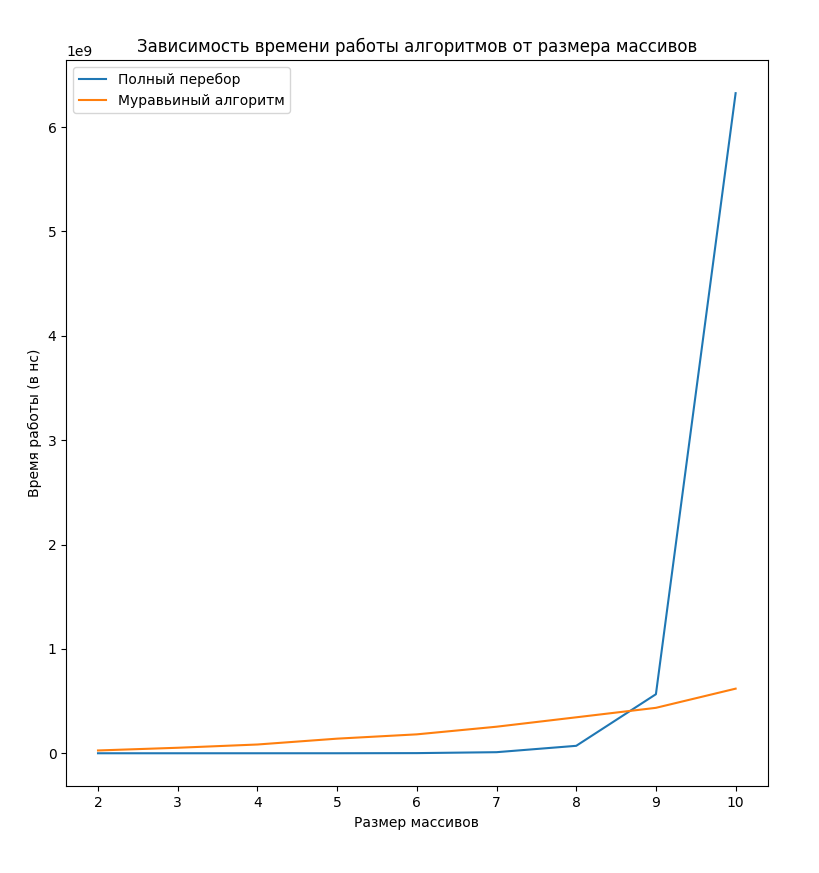
\includegraphics[width=\linewidth]{inc/graph.png}
	\end{center}
	\caption{График зависимости времени работы алгоритмов от размера матрицы}
\end{figure}
\FloatBarrier


Результаты тестирования второго случая представлены в таблице 4.2.
Полная таблица результатов представлена в приложении 1.
В первых пяти столбцах -- параметры муравьиного алгоритма, в шестом -- выдаваемый результат, в седьмом -- ошибка.

\FloatBarrier
\begin{table}[h]
	\caption{Результаты тестов}
	\centering
	\begin{tabular}{ | l | l | l | l | l | l | l |}
		\hline
		$\alpha$ & $\beta$ & Q & p & max\_iter & Результат & Ошибка \\ 
		\hline
1 & 1 & 1 & 0.5 & 10 & 804 & 212 \\ 
1 & 1 & 1 & 0.5 & 1000 & 592 & 0 \\ 
1 & 1 & 5 & 0.5 & 10 & 681 & 89 \\ 
1 & 1 & 5 & 0.5 & 1000 & 592 & 0 \\ 
1 & 2 & 1 & 0.5 & 10 & 705 & 113 \\ 
1 & 2 & 1 & 0.5 & 1000 & 592 & 0 \\ 
1 & 2 & 5 & 0.5 & 10 & 592 & 0 \\ 
1 & 2 & 5 & 0.5 & 1000 & 705 & 113 \\ 
1 & 3 & 1 & 0.5 & 10 & 592 & 0 \\ 
1 & 3 & 1 & 0.5 & 1000 & 683 & 91 \\ 
2 & 1 & 1 & 0.5 & 10 & 592 & 0 \\ 
2 & 1 & 1 & 0.5 & 1000 & 592 & 0 \\ 
2 & 1 & 5 & 0.5 & 10 & 672 & 80 \\ 
2 & 1 & 5 & 0.5 & 1000 & 592 & 0 \\ 
2 & 2 & 1 & 0.5 & 10 & 705 & 113 \\
2 & 2 & 1 & 0.5 & 1000 & 592 & 0 \\  
2 & 3 & 1 & 0.5 & 10 & 592 & 0 \\ 
2 & 3 & 1 & 0.5 & 1000 & 705 & 113 \\ 
2 & 3 & 5 & 0.5 & 10 & 592 & 0 \\ 
2 & 3 & 5 & 0.5 & 1000 & 592 & 0 \\  
3 & 2 & 1 & 0.5 & 10 & 592 & 0 \\ 
3 & 2 & 1 & 0.5 & 1000 & 592 & 0 \\ 
3 & 2 & 5 & 0.5 & 10 & 592 & 0 \\ 
3 & 2 & 5 & 0.5 & 1000 & 683 & 91 \\ 
3 & 3 & 1 & 0.5 & 10 & 592 & 0 \\ 
3 & 3 & 1 & 0.5 & 1000 & 592 & 0 \\ 
3 & 3 & 5 & 0.5 & 10 & 683 & 91 \\ 
3 & 3 & 5 & 0.5 & 1000 & 663 & 71 \\ 
		\hline
\end{tabular}
\end{table}
\FloatBarrier


В 72 случаев из 108 программа выдавала правильный результат.

Проанализируем ошибки. В таблице 4.3 приведены сведения о средней ошибке в зависимости от количества итераций.

\FloatBarrier
\begin{table}[h]
	\caption{Результаты тестов}
	\centering
	\begin{tabular}{ | l | l | l |}
		\hline
		Количество итераций & Количество ошибок & Средняя ошибка \\ 
		\hline
		10 & 17 & 51.84 \\
		100 & 10 & 27 \\
		1000 & 9 & 23.47 \\
		\hline
	\end{tabular}
\end{table}
\FloatBarrier

Видно, что с ростом количества итераций количество ошибок и средняя ошибка падают.
От значения остальных параметров зависимостей не обнаружено, что о говорит о том,
что значения параметром должны регулироваться в зависимости от задачи.

Лучшие параметры - параметры, у которых в столбце ошибок значение 0.
Например, лучшей комбинации аргументов соответствует строка 2 в таблице 4.3.
Полный список параметров, при котором программа выдаёт правильный ответ, можно увидеть в приложении 1.

\section{Вывод}
Применимость алгоритмов зависит от того, насколько велик размер матрицы расстояний.
При размере $ N < 9 $ алгоритм полного перебора работает быстрее, чем муравьиный алгоритм.
При $ N = 2 $ перебор быстрее в 275 раз, а при $ N = 8 $ в 4 раза.
Но при дальнейшем увеличении матрицы муравьиный алгоритм работает быстрее.
При $ N = 12 $ муравьиный алгоритм превосходит перебор в 82 раза.
При $ N > 12 $ время для подбора подсчитать не удалось -- оно слишком велико.

Муравьиный алгоритм при различных параметрах выдаёт разные ответы.
Регулировка параметров производится вручную, и значения параметров зависят от задачи.